\documentclass[acmart]{apa6}

\usepackage{amssymb,amsmath}
\usepackage{ifxetex,ifluatex}
\usepackage{fixltx2e} % provides \textsubscript
\ifnum 0\ifxetex 1\fi\ifluatex 1\fi=0 % if pdftex
  \usepackage[T1]{fontenc}
  \usepackage[utf8]{inputenc}
\else % if luatex or xelatex
  \ifxetex
    \usepackage{mathspec}
    \usepackage{xltxtra,xunicode}
  \else
    \usepackage{fontspec}
  \fi
  \defaultfontfeatures{Mapping=tex-text,Scale=MatchLowercase}
  \newcommand{\euro}{€}
\fi
% use upquote if available, for straight quotes in verbatim environments
\IfFileExists{upquote.sty}{\usepackage{upquote}}{}
% use microtype if available
\IfFileExists{microtype.sty}{\usepackage{microtype}}{}

% Table formatting
\usepackage{longtable, booktabs}
\usepackage{lscape}
% \usepackage[counterclockwise]{rotating}   % Landscape page setup for large tables
\usepackage{multirow}		% Table styling
\usepackage{tabularx}		% Control Column width
\usepackage[flushleft]{threeparttable}	% Allows for three part tables with a specified notes section
\usepackage{threeparttablex}            % Lets threeparttable work with longtable

% Create new environments so endfloat can handle them
% \newenvironment{ltable}
%   {\begin{landscape}\begin{center}\begin{threeparttable}}
%   {\end{threeparttable}\end{center}\end{landscape}}

\newenvironment{lltable}
  {\begin{landscape}\begin{center}\begin{ThreePartTable}}
  {\end{ThreePartTable}\end{center}\end{landscape}}

  \usepackage{ifthen} % Only add declarations when endfloat package is loaded
  \ifthenelse{\equal{\string acmart}{\string man}}{%
   \DeclareDelayedFloatFlavor{ThreePartTable}{table} % Make endfloat play with longtable
   % \DeclareDelayedFloatFlavor{ltable}{table} % Make endfloat play with lscape
   \DeclareDelayedFloatFlavor{lltable}{table} % Make endfloat play with lscape & longtable
  }{}%



% The following enables adjusting longtable caption width to table width
% Solution found at http://golatex.de/longtable-mit-caption-so-breit-wie-die-tabelle-t15767.html
\makeatletter
\newcommand\LastLTentrywidth{1em}
\newlength\longtablewidth
\setlength{\longtablewidth}{1in}
\newcommand\getlongtablewidth{%
 \begingroup
  \ifcsname LT@\roman{LT@tables}\endcsname
  \global\longtablewidth=0pt
  \renewcommand\LT@entry[2]{\global\advance\longtablewidth by ##2\relax\gdef\LastLTentrywidth{##2}}%
  \@nameuse{LT@\roman{LT@tables}}%
  \fi
\endgroup}


  \usepackage{graphicx}
  \makeatletter
  \def\maxwidth{\ifdim\Gin@nat@width>\linewidth\linewidth\else\Gin@nat@width\fi}
  \def\maxheight{\ifdim\Gin@nat@height>\textheight\textheight\else\Gin@nat@height\fi}
  \makeatother
  % Scale images if necessary, so that they will not overflow the page
  % margins by default, and it is still possible to overwrite the defaults
  % using explicit options in \includegraphics[width, height, ...]{}
  \setkeys{Gin}{width=\maxwidth,height=\maxheight,keepaspectratio}
\ifxetex
  \usepackage[setpagesize=false, % page size defined by xetex
              unicode=false, % unicode breaks when used with xetex
              xetex]{hyperref}
\else
  \usepackage[unicode=true]{hyperref}
\fi
\hypersetup{breaklinks=true,
            pdfauthor={},
            pdftitle={Do self-reported motivation measures or behavioral traces matter more? Exploring predictors of achievement in online science classes},
            colorlinks=true,
            citecolor=blue,
            urlcolor=blue,
            linkcolor=black,
            pdfborder={0 0 0}}
\urlstyle{same}  % don't use monospace font for urls

\setlength{\parindent}{0pt}
%\setlength{\parskip}{0pt plus 0pt minus 0pt}

\setlength{\emergencystretch}{3em}  % prevent overfull lines


% Manuscript styling
\captionsetup{font=singlespacing,justification=justified}
\usepackage{csquotes}
\usepackage{upgreek}



\usepackage{tikz} % Variable definition to generate author note

% fix for \tightlist problem in pandoc 1.14
\providecommand{\tightlist}{%
  \setlength{\itemsep}{0pt}\setlength{\parskip}{0pt}}

% Essential manuscript parts
  \title{Do self-reported motivation measures or behavioral traces matter more?
Exploring predictors of achievement in online science classes}

  \shorttitle{Predictors of achievement}


  \author{Emily Bovee\textsuperscript{1}, Joshua Rosenberg\textsuperscript{2}, \& John Ranellucci\textsuperscript{3}}

  % \def\affdep{{"", "", ""}}%
  % \def\affcity{{"", "", ""}}%

  \affiliation{
    \vspace{0.5cm}
          \textsuperscript{1} Michigan State University\\
          \textsuperscript{2} University of Tennessee, Knoxville\\
          \textsuperscript{3} Hunter College  }

  \authornote{
    Correspondence concerning this article should be addressed to Emily
    Bovee, . E-mail:
    \href{mailto:ebovee@msu.edu}{\nolinkurl{ebovee@msu.edu}}
  }


  \abstract{We used random forest modeling to explore predictors of virtual middle
school science students' achievement. Using a robust dataset that
includes behavioral trace data from the course learning management
system and self-reported indicators of students' academic motivation, we
examined which indicators were most predictive of achievement. Framed in
the Expectancy-Value Theory of academic motivation, we explored
students' perceived competence for science and their value for science
as potential predictors of achievement. We found that trace measures of
engagement with the discussion board more strongly predicted final
course grade than did indicators of science motivation.}
  \keywords{Science, motivation, random forest, machine learning, learning
management system, educational success, achievement \\

    
  }





\usepackage{amsthm}
\newtheorem{theorem}{Theorem}[section]
\newtheorem{lemma}{Lemma}[section]
\theoremstyle{definition}
\newtheorem{definition}{Definition}[section]
\newtheorem{corollary}{Corollary}[section]
\newtheorem{proposition}{Proposition}[section]
\theoremstyle{definition}
\newtheorem{example}{Example}[section]
\theoremstyle{definition}
\newtheorem{exercise}{Exercise}[section]
\theoremstyle{remark}
\newtheorem*{remark}{Remark}
\newtheorem*{solution}{Solution}
\begin{document}

\maketitle

\setcounter{secnumdepth}{0}



\section{1. INTRODUCTION}\label{introduction}

\enquote{Data-driven decision making} is implemented in different ways
at different schools, leading educators to hold divergent attitudes
about it (Ikemoto \& Marsh, 2007). Thus, there is a need to explore the
ways in which educators can most effectively collect and use data to
support student learning (Hamilton et al., 2009). One area of interest
is the delivery of online instruction, which is becoming more prevalent:
in 2007, over 3.9 million U.S. students were enrolled one or more online
courses (Allen \& Seaman, 2008). We use a robust data set, which
includes self-reported motivation as well as behavioral trace data
collected from a learning management system to identify predictors of
final course grade. Our work examines the idea of educational success in
terms of student interactions with an online science course. In the
current study, we examine the educational experiences of students in
online science courses at a virtual middle school in order to
characterize their motivation to achieve and their tangible engagement
with the course in terms of trace measures.

One meaningful perspective from which to consider students' engagement
with online courses is related to their motivation to achieve. More
specifically, it is important to consider how and why students are
engaging with the course. To consider the psychological mechanisms
behind achievement is valuable because doing so may help to identify
meaningful points of intervention for educators.

Expectancy-value theory (EVT) is a key motivational framework that
explains the reasons that students are motivated to achieve (Eccles et
al., 1983). EVT posits that students are motivated to achieve when (1)
they perceive themselves to be capable of success (e.g.,
\enquote{expectancy}) and (2) they perceive present or future value in
the task at hand (e.g., \enquote{value}). Two types of value are utility
value, which refers to the degree to which students perceive that a
given task will be useful to them for some future goal, and interest
value, which refers to the level of interest students have in a given
task. In this study, we will consider utility value, interest value, and
expectancy for success as predictors of student achievement.

We investigated three research questions:

\begin{enumerate}
\def\labelenumi{\arabic{enumi}.}
\tightlist
\item
  Is motivation - operationalized as interest value, utility value and
  perceived competence for science - relatively more predictive of
  course grades as compared to other online indicators of engagement?
\item
  Which type of motivation (e.g., interest value, utility value, and
  perceived competence) is most predictive of achievement?
\item
  Which type of trace measures (e.g., time spent on course and those
  associated with participating on discussion boards) is most predictive
  of achievement?
\end{enumerate}

\section{2. METHOD}\label{method}

\subsection{2.1 Participants}\label{participants}

Participants were 499 students enrolled in online middle school science
courses in 2015-2016.

\subsection{2.2 Setting / Data Sources}\label{setting-data-sources}

The setting of this study was a public, provider of individual online
courses in a Midwestern state. In particular, the context was two
semesters (Fall and Spring) of offerings of five online science courses
(Anatomy \& Physiology, Forensic Science, Oceanography, Physics, and
Biology), with a total of 36 classes. Students completed a pre-course
survey about their self-reported motivation in science --- in
particular, their perceived competence, utility value, and interest. We
also kept track of the time students spent on the course (obtained from
the Learning Management System) and their final course grades as well as
their involvement in discussion forums. For the discussion board data,
we used the Linguistic Inquiry and Word Count (LIWC; Pennebaker, Boyd,
Jordan, \& Blackburn, 2015) to calculate the number of posts per student
and variable for the mean levels of students' cognitive processing,
positive affect, and social-related discourse evidenced by their posts.

\subsection{2.3 Procedure}\label{procedure}

At the beginning of the semester, students were asked to complete the
pre-course survey about their perceived competence, utility value, and
interest. At the end of the semester, the time students spent on the
course, their final course grades, and the contents of the discussion
forums were collected.

\subsection{2.5 Preliminary data
analysis}\label{preliminary-data-analysis}

The random forest algorithm does not accept cases with missing data.
Thus, we deleted cases listwise if data were missing. This decision
eliminated 51 cases from our original data set, to bring us to our final
sample size of 499 unique students.

\subsection{2.6 Data analysis for main
models}\label{data-analysis-for-main-models}

For our analyses, we used Random Forest modeling (Breiman, 2001). Random
forest is an extension of decision tree modeling, whereby a collection
of decision trees are simultaneously \enquote{grown} and are evaluated
based on out-of-sample predictive accuracy (Breiman, 2001). Random
forest is random in two main ways: first, each tree is only allowed to
\enquote{see} and split on a limited number of predictors instead of all
the predictors in the parameter space; second, a random subsample of the
data is used to grow each individual tree, such that no individual case
is weighted too heavily in the final prediction.

Whereas some machine learning approaches (e.g., boosted trees) would
utilize an iterative model-building approach, random forest estimates
all the decision trees at once. In this way, each tree is independent of
every other tree. Thus, the random forest algorithm provides a robust
regression approach that is distinct from other modeling approaches. The
final random forest model aggregates the findings across all the
separate trees in the forest in order to offer a collection of
\enquote{most important} variables as well as a percent variance
explained for the final model.

A random forest is well suited to the research questions that we had
here because it allows for nonlinear modeling. We hypothesized complex
relationships between students' motivation, their engagement with the
online courses, and their achievement. For this reason, a traditional
regressive or structural equation model would have been insufficient to
model the parameter space we were interesting in modeling. Our random
forest model had one outcome and eleven predictors. A common tuning
parameter for machine learning models is the number of variables
considered at each split (Kuhn, 2008): We considered three variables at
each splot for this analysis.

The outcome was the final course grade that the student earned. The
predictor variables included motivation variables (interest value,
utility value, and science perceived competence) and trace variables
(the amount of time spent in the course, the course name, the number of
discussion board posts over the course of the semester, the mean level
of cognitive processing evident in discussion board posts, the positive
affect evident in discussion board posts, the negative affect evident in
discussion board posts, and the social-related discourse evident in
their discussion board posts). We used this random forest model to
address all three of our research questions.

In this study, we used the package randomForest in R (Liaw, 2018). 500
trees were grown as part of our random forest. We partitioned the data
before conducting the main analysis so that neither the training and
testing data set would not be disproportionately representative of
high-achieving or low-achieving students. The training data set
consisted of 80\% of the original data (\emph{n} = 400 cases), whereas
the testing data set consisted of 20\% of the original data (\emph{n} =
99 cases). We built our random forest model on the training data set,
and then evaluated the model on the testing data set. Three variables
were tried at each node. To interpret our findings, we examined three
main things: (1) predictive accuracy of the random forest model, (2)
variable importance, and (3) variance explained by the final random
forest model.

\section{3. RESULTS}\label{results}

First, we assessed the model based calculations specific to the data
used to fit the model. Using the data in the training set (with \emph{n}
= 400 observations), we calculated the \(R^2\) value, indicating the
proportion of the variability in the outcome (final grade) accounted for
by the nine predictor variables. The \(R^2\) value was .528, which
suggested that for this sample and partition of the data, just more than
one-half of the variability in the outcome could be attributed to the
predictors that were included.

In addition to using the training data set to calculate the \(R^2\)
value, as we used a training and a test (with \emph{n} = 99
observations) data set, we were able to compare how well model predicted
the outcome, students' final grade. Thus, the predictive accuracy of our
random forest model was assessed by examining the difference between the
predicted values for the testing data set and the actual values. Using
the 99 test set observations and their predictions, we calculated the
Root Mean Square Error (RMSE), which was 12.70. Given that students'
final grades were measured on a 0-100 scale, this represents, in
substantive terms, modest - but not excellent - predictive accuracy
(especially given that the \emph{SD} for students' final grade in the
test set was 19.50).

We also visually compared students' observed (or actual) and their
predict final grades, as in Figure 2. This helped us to see that while
the model predicted the final grade accurately overall
(\(M_{\text{observed-final-grade}}\) = 78.69;
\(M_{\text{predicted-final-grade}}\) = 78.83), the model predicted
grades closer to the mean more frequently than as observed in the
training data set and predicted very high grades less frequently than
observed in the training data set.

\begin{figure}
\centering
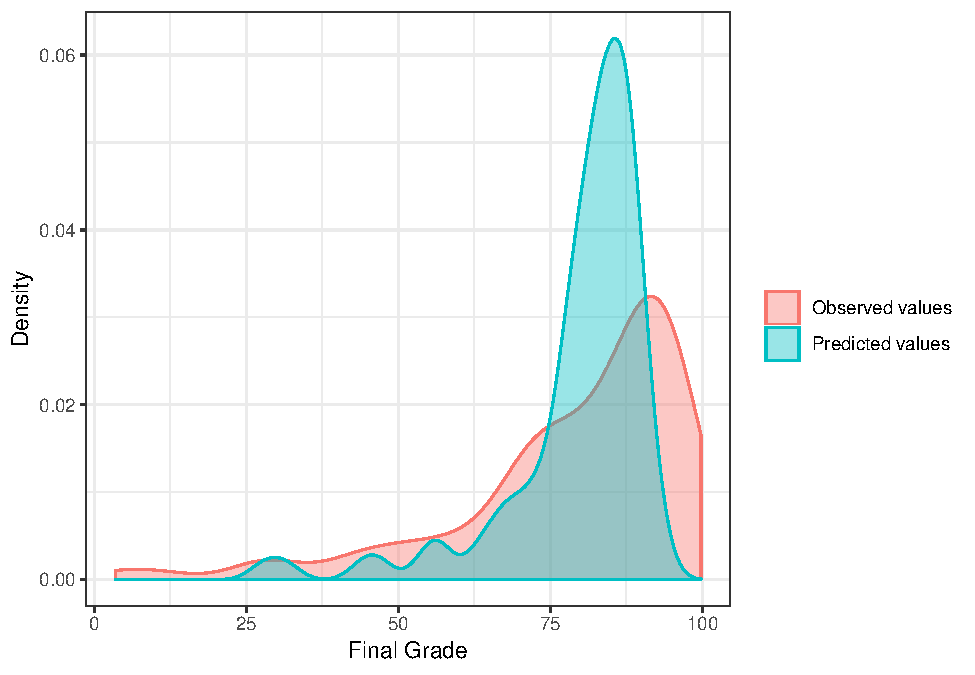
\includegraphics{LAK_Manuscript_files/figure-latex/unnamed-chunk-3-1.pdf}
\caption{\label{fig:unnamed-chunk-3}Distribution of students' observed
(actual) and predicted final grade}
\end{figure}

Below, we will discuss in detail the specific findings for each of our
research questions, which concern the variable importance plots.
Variable importance plots are interpreted based on the incremental
percent change in mean-squared-error (MSE) if a given variable is
scrambled in the original data set (James, Witten, Hastie, \&
Tibshirani, 2013). In other words, variable importance plots help to
answer the question: if a variable is scrambled so as not to relate to
the outcome in any systematic way, how much does this randomization
affect the mean squared error? If a variable's scrambling results in a
large change in MSE, it is thought to be more important.

\subsection{Results for Research Question
1}\label{results-for-research-question-1}

Research question 1 asked whether motivation was a better predictor of
achievement than behavioral engagement indicators. With respect to
research question 1, the variable importance plot for final grade
indicated that the change in mean squared error was more strongly
affected by trace variables than motivation measures. The most
predictive variable was the number of discussion posts, followed by the
amount of time spent in the course. The course identifier, evidence for
negative affect in the discussion posts, and level of cognitive
processing associated with the discussion posts were the predictors that
were next in terms of importance. All of these predictors were more
important than all of the motivation variables.

\subsection{Results for Research Question
2}\label{results-for-research-question-2}

Research question 2 asked which of the motivation variables was most
predictive of course achievement. As presented in Table 1, among
motivation variables, utility value was most important, followed by
perceived competence. Interest value was the least predictive of the
motivation variables; indeed, interest value was the least predictive of
all variables in the random forest model.

\begin{figure}
\centering
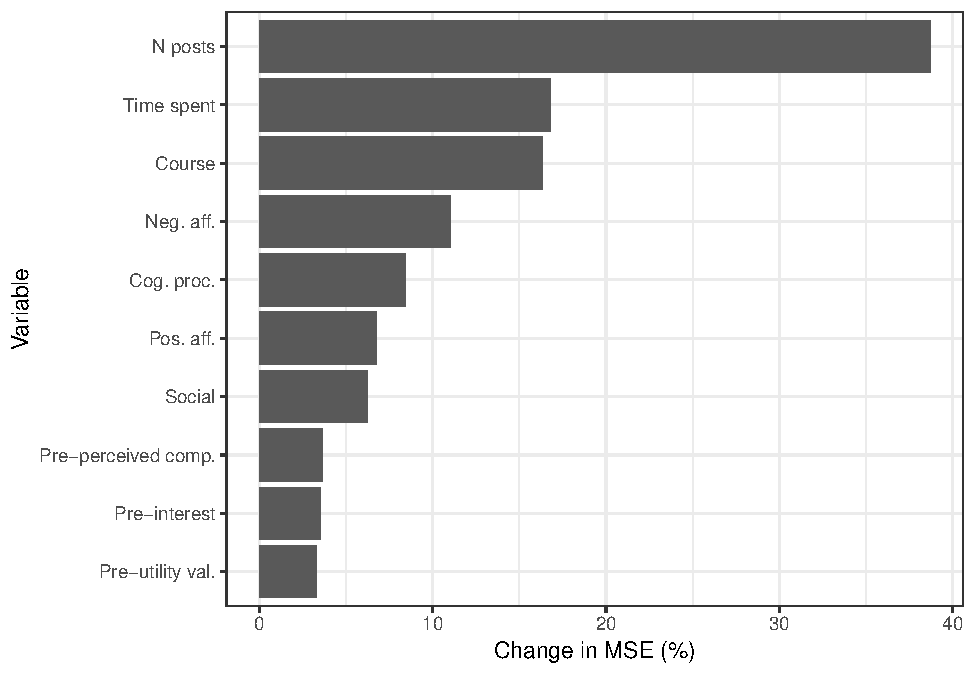
\includegraphics{LAK_Manuscript_files/figure-latex/unnamed-chunk-4-1.pdf}
\caption{\label{fig:unnamed-chunk-4}Variable importance (change in Mean
Square Error {[}MSE{]})}
\end{figure}

\subsection{Results for Research Question
3}\label{results-for-research-question-3}

Research question 3 asked which of the trace variables was most
predictive of course achievement. The most predictive variable in terms
of achievement was the number of posts in the discussion forums. Given
its importance, we sought to explore how the strength of relation
between students' predicted and observed final grade might vary as a
function of the number of posts. We turned the number of posts into a
categorical variable with three levels and examined whether the
relationship between students' predicted and observed final grade
appeared to differ.

\begin{figure}
\centering
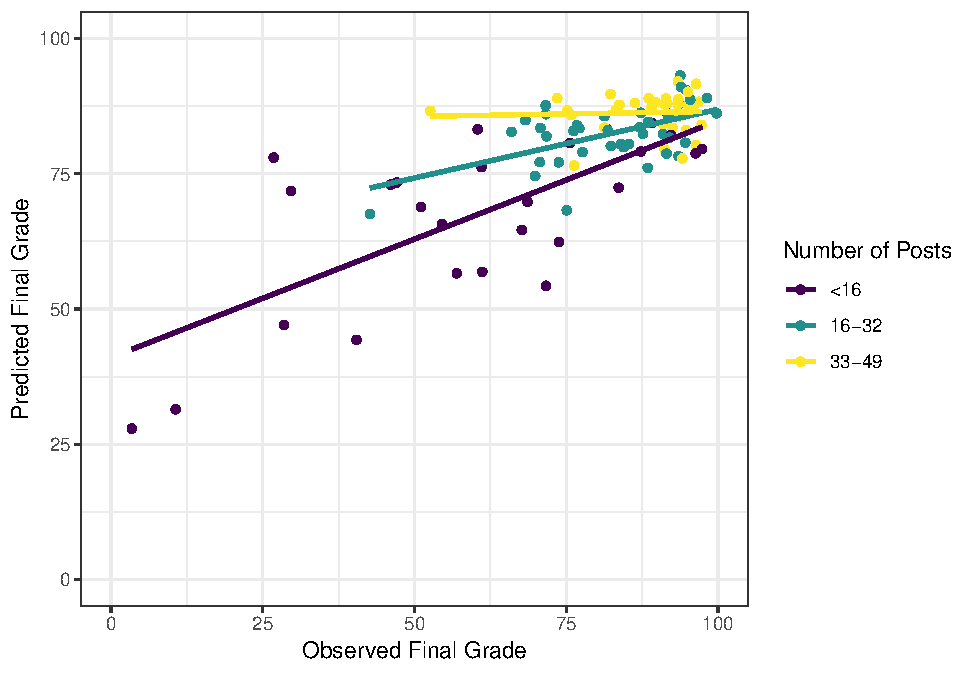
\includegraphics{LAK_Manuscript_files/figure-latex/unnamed-chunk-5-1.pdf}
\caption{}
\end{figure}

For the 99 observations in the test dataset, this figure revealed there
to be a stronger relationship between the predicted and observed final
grade for students who posted fewer times to the discussion forum. For
students with the most posts (between 33 and 49), the relationship
appeared to be nearly zero, suggesting that \emph{other} (important)
variables mattered more for these students (or that the model was
predicting these students' final grades poorly, a postsibility given
that the model appeared to predict the final grades of the students with
the highest final grades poorly).

The number of posts to the discussion forum by students was the most
predictive of all the variables in the model, followed by the time
students spent on the course. After the course students were in (not
considered a trace measure), the negative affect evidenced by students'
discussion forum posts and the extent of the cognitive processing
evidenced by them were the next most important.

\section{4. DISCUSSION}\label{discussion}

Overall, our random forest model explained a large amount of the
variance in achievement in this study (e.g., 55.49\%). However, the
predictive accuracy of the model might ideally be higher: the absolute
value of the average difference between the predicted final grade and
actual final grade was 11.8\%. This discrepancy suggests that whereas
our model did a good job at explaining variance in the outcome of
achievement, it did not perform as well in its prediction of
\enquote{unseen} test data as would be ideal. Future research should
thus explore whether the predictive accuracy of the model could be
further developed. Even so, our predictive accuracy is not so low as to
be unhelpful. Rather, this study offers interesting insights as to the
relative importance of motivation constructs and trace measures of
engagement in terms of explanatory power in explaining middle school
students' online science course grades.

Surprisingly, we found that trace measures of engagement with a learning
management system were more predictive of student achievement than
motivation variables.

\subsection{Limitations}\label{limitations}

This study was limited in some important ways. First, we chose to
operationalize achievement as final course grade. Future work could
examine other meaningful outcomes. Additionally, we did not account for
the number of discussion posts that were required in a given course and
it is important that future research endeavor to explore whether this
plays a role in predicting the outcome.

\subsection{Implications}\label{implications}

As more and more courses move online, data will continue to accumulate
at rapid rates. It is important that educators and administrators
consider the implications of computer-mediated instruction. This study
suggests that the measurement of students' engagement with courses is
helpful in understanding their achievement in these courses. Trace data
is valuable to collect and it could be valuable for educators to
consider it more thoroughly. This study also offers implications in
terms of the motivation constructs studied. The importance of the
engagement with the course through discussion board posts in terms of
predicting final grade suggests that perhaps it is valuable for students
to post even if they are not intrinsically motivated to do so. Future
research should explore the complex relations between student motivation
and course engagement, especially insofar as to examine characteristics
of the online experience that could make these relations different than
the patterns of relations that would be evident in a face-to-face
classroom.

\section{References}\label{references}

\begingroup
\setlength{\parindent}{-0.5in} \setlength{\leftskip}{0.5in}

Allen, I. E. \& Seaman, J. (2008). \emph{Staying the course: online
education in the United States}. Needham, MA: Sloan Consortium.

Breiman, L. (2001). \emph{Random forests. Machine Learning, 45}, 5--32.
\url{doi:10.1023/A:1010933404324}

Hamilton, L., Halverson, R., Jackson, S., Mandinach, E., Supovitz, J.,
\& Wayman, J. (2009). \emph{Using student achievement data to support
instructional decision making (NCEE 2009-4067).} Washington, DC:
National Center for Education Evaluation and Regional Assistance,
Institute of Education Sciences, U.S. Department of Education. Retrieved
from \url{http://ies.ed.gov/ncee/wwc/PracticeGuide.aspx?sid=12}

Ikemoto, G. S., \& Marsh, J. A. (2007). Cutting through the
\enquote{data driven} mantra: Different conceptions of data-driven
decision making. In P.A. Moss (Ed.), \emph{Evidence and decision making}
(National Society for the Study of Education Yearbook, Vol. 106, Issue
1, pp.~105--131). Chicago, IL: National Society for the Study of
Education.

James, G., Witten, D., Hastie, T., \& Tibshirani, R. (2013). \emph{An
introduction to statistical learning}. New York, NY: Springer.

Kuhn, M. (2008). Caret package. \emph{Journal of Statistical Software,
28}(5), 1-26.

Liaw, A. (2018). \emph{Package \enquote{randomForest}: Breiman and
Cutler's Random Forests for Classification and Regression.}
\url{https://cran.r-project.org/web/packages/randomForest/randomForest.pdf}

Pennebaker, J.W., Boyd, R.L., Jordan, K., \& Blackburn, K. (2015).
\emph{The development and psychometric properties of LIWC2015.} Austin,
TX: University of Texas at Austin.

\hypertarget{refs}{}

\endgroup






\end{document}
